\documentclass{CRPITStyle} 
%\usepackage{epsfig}   % Packages to use if you wish
%\usepackage{lscape}   % 
\usepackage[authoryear]{natbib}

\usepackage{ifpdf}
\usepackage[utf8]{inputenc}
\usepackage{cite}
\usepackage{paralist}
\usepackage[pdftex]{graphicx}
\usepackage{caption}
\usepackage{subcaption}
\graphicspath{{.}{images/}} 
\DeclareGraphicsExtensions{.jpg}
\usepackage[cmex10]{amsmath}
\usepackage[rgb]{xcolor}
\usepackage{natbib}


\newcommand*{\bd}[1]{\multicolumn{1}{|c|}{\bfseries #1}}
\renewcommand{\cite}{\citep}
\pagestyle{empty}
\thispagestyle{empty}
\hyphenation{roddick}

\begin{document}

\title{Securing WSN update from Intrusion using Time Signature of Over the Air Update Protocol}
\author{A S M Ashraful Alam  \and  David Eyers 	  }
\affiliation{Department of Computer Science, University of Otago, New Zealand\\
			Email:~{\tt \{aalam, dme\}@cs.otago.ac.nz} 	}

\maketitle

\newcommand\conferencenameandplace{13th Australasian Symposium on Parallel and Distributed Computing (AusPDC 2015), Sydney, Australia, January 2015}
      \newcommand\volumenumber{163}
      \newcommand\conferenceyear{2015}
      \newcommand\editorname{Bahman Javadi and Saurabh Kumar Garg}
      \toappearstandard 


\begin{abstract}
While over the air (OTA) software updates makes certain WSN management tasks easy, they are vulnerable to intrusion attempts.
An adversary can take advantage of the resource-constrained nature of the sensor motes to break through the limited protection the sensors have.
To deal with this problem, we have suggested a passive security mechanism---an IDS that works on a timing analysis principle.  
\end{abstract}
\vspace{.1in}

\noindent {\em Keywords:} Sensor, Wireless Sensor Network, WSN, Intrusion Detection System, IDS, Security

\section{Introduction}
\label{sec:intro}

Wireless sensors or motes are deployed in large numbers in uncontrolled environments, which makes them difficult to manage.
Tasks such as bug-fixing are often managed using over the air (OTA) software update protocols such as Deluge~\cite{1031506}.
There are risks and vulnerabilities associated with Wireless Sensor Network (WSN) OTA software updates that can enable an attacker to steal sensitive information, log network events, or cause denial of service~\cite{1127826}.
%While OTA update protocols make certain WSN management tasks easy, they open up potential vulnerabilities.
An adversary can take advantage of the resource-constrained nature of the sensor motes to break through the limited protection that they have.
%and employ enough resources to break in through the limited protection the sensors are armed with.
% <dme> I generally think it's best form not to repeat sentences within body text and the abstract---I rephrase such repeated content. <Ash> okay

Security threats to WSNs are different in nature from threats to the Internet or even other wireless technologies. %technology. % and ad-hoc network, MANET.
Implementation of security techniques in WSNs are characterised by constrained resources.
%Wireless channels are inherently considered to be less secure.
As a result, well developed cryptographic security mechanisms such as WPS and PKM are inappropriate.
% <dme> you haven't said why <Ash> connected
Wireless channels offer little physical protection.
Moreover, the capability of computing devices that can computationally compromise the cryptographic protection in sensors is growing rapidly.
% at much faster rate.
% <dme> you can't say things like "much faster rate" unless you also say what you're comparing against! <Ash> okay
As a result, WSNs are more vulnerable to intrusion attempts and security threats from attackers.
%However, the simple communication protocols and design make it easy to perform intrusion detection in WSNs~\cite{quing09}.
% <dme> it's not obvious why. <Ash> I'll look through the reference again. I think the author hasn't explained it either
An Intrusion Detection System (IDS) can detect  break-in events and raise alerts, possibly also estimating the location and extent of the problem. % following some predefined procedures. 
%It may be able to report the location and extent of break-in as well.


Proposed IDS techniques vary greatly in their approaches.
Misuse-based  detection  techniques aim to detect known attacks by identifying undesired activities based on usage signatures.
However, they are ineffective against previously-unseen attacks and 
may wrongly identify legitimate activities as an intrusion because of similarities to existing signatures.
Conversely, anomaly-based IDSs build statistical signatures based on a definition of normal activity.
Unfortunately, a system may display previously unknown behaviour e.g., rare critical events like earthquakes or tsunamis may raise false positive intrusion alerts within environmental monitoring sensors.
On the other hand, an intrusion that masks its pattern under the hood of normal behaviour, for example: increased packet traffic during OTA update, would go undetected.
Specification-based and reputation-based techniques rely on manual input for defining normal and anomalous behaviour with lesser reliance on automation.
However, these techniques have not been proved to be very effective because human interaction are more prone to errors and require more learning time~\cite{quing09, 1593102, 1290173, Chen:2009:NMI:1516241.1516282}. 
% <dme> previous sentence doesn't explain what it's talking about or prove its point.
%Although approaches described above   <Ash> I'll look through the reference again
%Despite innovative ideas, only few IDSs are able to address the security issues related to software update.
% <dme> the previous sentence didn't seem to add anything, so I removed it. ,<Ash> okay

Onat and Miri present an IDS design in which each node builds up statistics about received packets from its neighbours.
% based on the last N packets received from each neighbour.
If packets received from any neighbour display anomalous patterns after a predefined number of consecutive packets, intrusion alarms may be raised \cite{1512911}.
Unfortunately, packet count statistics are not suitable in OTA software update scenarios due to the significant increase in packet traffic from the update itself.
% <dme> it's the same idea though: just record the statistics during a software update. Why can't their methods be applied almost directly in the model you've built?
%<Ash> Well, software update is a decentralised process and works on a single hop basis. A node can receive pages and packets from different sources, it may need to discard duplicates, re-request some packet or even page for corrupt packaets and so many uncertainities. So, it may not be possible to establish an expected pattern. 
%Yet we can look into this type of processing.
However, this statistical treatment motivates us to employ timing analysis within OTA update protocols.

In this paper, we present an IDS that can detect intrusion in case of WSN software update.
The algorithm requires update protocol to send back a datagram containing the update time to work out a `Surprise Score' or `Intrusion Warning Score' (IWS)~\cite{aalam15}.
Our main contributions are: 
the technique identifies anomalies in software update patterns and scores them quantitatively;
we demonstrate that simulation can indicate the positions of WSN nodes that will best support the ability of similar IDSs to detect anomalies. 
%scheme i.e., the IDS expectations can provide useful insight for designing secure WSN.
The rest of this paper is organised as follows.
In Section~\ref{sec:meth}, we give a brief overview of the system  design and the experiment methodology. 
Then we analyse the experimental results and present our evaluation in Section~\ref{sec:eval}.  
Finally, we conclude our arguments in Section~\ref{sec:concl}.
%\vspace{-5mm}
%\rule{5mm}{5mm}

\section{Methodology}
\label{sec:meth}

\subsubsection*{System Design}
%The IDS framework components has been shown in \ref{fig:ids_fw}.
The IDS has three kinds of components---%
i) motes in radio network; 
ii) an IDS transport client (ITC) application in the sink; and
iii) an IDS application that runs on an system with higher resources, coordinates with ITC, remains physically attached to the sink, and houses a network database (NDB).

Following activities are necessary for the intrusion detection technique to work---%
i) Deluge protocol initiates update;
ii) Deluge disseminates the new software image using a multi-hop relay mechanism; 
iii) nodes deliver a datagram to the sink containing their timing information;
iv) packets from the nodes rely on other nodes \emph{en route} to reach to the sink; and
v) the ITC application in the sink delivers relevant information to the IDS for processing 

After checking for correctness, the ITC then inserts the update time and mote ID into the NDB in the IDS.
The IDS maintains an identifier to differentiate among different update times from different runs for the same mote.
The IDS uses timing measurements from authenticated initial software update runs to build signatures.
The time analyser module in the IDS inspects the NDB once an update activity has been detected. 
It determines the changes from the signature and calculates IWS based on following utility function:
\begin{equation}
\label{eqn2} 
	\mathit{IWS} = \sum \limits_{i=0}^{n} \frac{\left| \mu_i - t_i \right|}{\sigma_i + 1}
\end{equation}
where, 
$\mathit{i}$---mote index; %\notedme{Why were you using capital letters all through here?}  
$\mathit{t_i}$---image update time at mote $\mathit{i}$;  
$\mathit{\mu_i}$---mean update time at mote $\mathit{i}$;  and 
$\mathit{\sigma_i}$---standard deviation of update time at mote $\mathit{i}$. 

The system has been described elaborately in~\cite{aalam15}.

\subsubsection*{Threat Model}
%The threat model is directed towards injection of unauthorised program images to infect the entire WSN.
% <dme> I don't understand the previous sentence
The IDS is expected to handle malicious node update attempts, node compromise, and node failure.
We assume that an  attacker  can take over one or more nodes deployed in hostile environment, access the code in a compromised node, and use cryptanalysis to represent a false identity without physically compromising a node.
% <dme> you need to make the layers of the system clear. It sounds like the OS can be compromised from the previous text, but that isn't the aim, is it?
However, he has  no special  access to  the  network and is unable to modify the underlying protocols running in the uncompromised nodes.
We assume a static WSN with a single  sink that cannot be compromised. All motes are assumed to have time synchronisation accurate to 1~$\mu$s, e.g., using TSMP. %~\cite{Pister08tsmp:time}.
\subsubsection*{Experiment Settings}
\label{subsec:sim_env} 
We used `Cooja'---a %\footnote{https://github.com/contiki-os/contiki/wiki/An-Introduction-to-Cooja}, a 
 network simulator in Contiki v2.7 running on Ubuntu 12.04, to simulate the software update pattern associated with Deluge protocol.
The simulations evaluated the IDS in different WSN topologies and explored the effect of parameters such as power level.
Evaluating the IDS on each of the topologies consisted of several test runs that  were of two kinds: 
aimed at building signatures consisting of 20 individual simulations initiated from the sink; and
simulations that replicated intrusion from nodes other than the sink.
We explored different  topologies such as: linear, circular, elliptical, double rings, wide line, grid, tree and other random topologies, but do not have space to discuss them in detail here. %describe them all.
The motes were placed at a distance of 30--35 meters to allow  multiple transmission paths to all motes. 
For most experiments, the radio transmission power level was set at 100\% which has an approximate maximum effective transmission range of 50 meters and is able to interfere with other motes up to 100 meters away.
The `Owheo WSN'\footnote{WSN deployed in the Owheo Building at the University of Otago. It is intended to be used for research purposes.} topology was additionally tested at 50\% power level.%  to observe the difference from the parameter change.

\subsection*{Experimental Procedure}
\label{subsec:proc}
\paragraph*{Step 1} All motes in the WSN were booted up at same time running one version of a diagnostic application that reports its time, version number and mote ID every second on its serial terminal. 
%Step 2: Stopping the simulation
\paragraph*{Step 2}  The sink dynamically began the update process by propagating another version of the software image using Deluge protocol. %, which is also called 
Whenever the transfer to a mote was complete, the new image would  reboot to begin executing.
In a real system, the modified Deluge protocol that runs with the OS would send a report datagram to the sink.
% <dme> what of the risks of doing this? I'm still concerned that you're "selling" a complete IDS when it might actually have some serious holes...
%<Ash> I have added the reference to use of similar technique in real system. I would suggest at least two alternative approaches that, I suppose, should work in real system e.g., use of AM packet and use of CTP.
%%<Ash> I feel "alarmed" when you use the word `concerned'. :(. Is it that bad? I want to use intrusion detection technique instead of IDS (I really agree it is not a complete IDS).
A similar technique has been employed  for WSN failure detection in real system by~\cite{Kam14}.
The simulator continued until all the motes in the WSN were updated and the times of their updates were logged. 
%The update time of each mote were filtered out  and were sorted In ascending order of update time.
% <dme> the previous point is too simple to mention, I think. <Ash> okay
\paragraph*{Step 3}  Processed data  were statistically treated to build the signature consisting of mean and standard deviation of  mote update time.
Changes to the topology or configuration of the WSN would necessitate recalibrating the signature.
\paragraph*{Step 4}   Intrusion attacks at different nodes were replicated in simulations.
The individual simulation runs were treated in a fashion  similar to~Step 1 and Step 2.
The update time recorded at each of the motes was then analysed using Equation~\ref{eqn2} to produce IWS.
The resulting values from this function presented an approximation of the abnormality of the new update pattern. The higher the IWS, the more unusual the pattern was. 
% <dme> You've failed to mention IWS in this step, which means readers will have no idea that the IWS scores you present later represent comparing an update initiated from their node, and measured from the real sink, compared to the baseline measurements.
%<Ash> Thank you very much. Without mentioning IWS, this portion was really incomplete
\paragraph*{Step 5}  We classified the IWS values into Intrusion Warning Zones (IWZ) based on a scale built from maximum expected IWS for a topology to imply certain warning levels.
% <dme> I'm not sure that I believe that the IWZ concept can work in practice, as we've discussed previously...
% <Ash> we devided into zones to associate some kind of classification of the scores. otherwise, the IWS itself is a quantitive measure
The heuristics follows from %statistical techniques and 
the feasibility of finding an easily identifiable boundary.
% <dme> don't understand what statistical techniques you're talking about 
% <Ash>statistical techniques meant the use of \mu and \sigma to calculate IWS in the  first palce
The IDS marks an IWS up to 10\% from the scale as GREEN to indicate safe zone,
10\%--30\% as GREY to indicate a situation where rules are not known and 
above 30\% to be possible intrusion and is marked as RED zone.
% <dme> what's the evidence for this making sense?
Forming IWZs requires the IDS to have knowledge of IWS for  intrusions at each individual node in the network.
% <dme> this doesn't sound feasible---I think you mean something slightly different... <Ash> rephrased correctly
Such knowledge can be built by replicating intrusion activity from the furthest few nodes.
% <dme> OK, that clears it up a bit, but it's not necessarily ALL possible intrusions. <Ash> rephrased correctly
% <dme> What's your proposed use for the IWZs anyway? I'm not sure the text covers this. <Ash> in this methodology I described what I did with the experiement. The utilization is in discussion section

\section{Results and Evaluation}
\label{sec:eval}

\begin{table*}[t!]
\centering
\begin{tabular}{|l|*{19}{r|}r|}
\hline
\bd{Node ID}           & \bd{1} & \bd{2} & \bd{3} & \bd{4} & \bd{5} & \bd{6} & \bd{7} & \bd{8} & \bd{9} & \bd{10} & \bd{11} & \bd{12} & \bd{13} & \bd{14} & \bd{15} & \bd{16} & \bd{17} \\% & \bd{18} & \bd{19} \\ % & \bd{20} \\
%Mote ID           & 1 & 2 & 3 & 4 & 5  & 6 & 7 & 8 & 9 & 10 & 11 & 12 & 13 & 14 & 15  & 16 & 17 & 18 & 19 & 20 \\
\hline
$\mu$            & 0 &19 & 79& 143&197 &268&340&404&466&539 &594 &547 &476 &408 &326 & 268&210 \\%& 152 & 83 \\ %& 19 \\
$\sigma$		 & 0 & 2 & 11 & 12 & 13 & 25& 27&31 &30 & 38 & 37 & 49 & 37 & 35 & 25  & 24 & 23 \\%& 24 & 16 \\ %& 3 \\
\hline
\end{tabular}
\caption{Statistics of mote update times in Double Ring topology (partial data presented)}
% <dme> time statistics of what? This is not usefully descriptive. <Ash> should be better now
\label{tab:stat_ellip}
\end{table*}

%In this section, we presents the results, their interpretation and evaluate the contribution.
%While discussing the performance and effects of the proposed IDS in different topologies are useful, discussing any of the topologies presents fair idea about the outcomes from the others and mentioning the cases when the outcome was considered  contrary to the expectations.

While evaluating all experimented topologies is useful, the results from Double Ring topology only is presented. %To suite space limitation
% and  exceptions in other topologies are mentioned.
% <dme> "exceptions in other topologies"---what does this mean? <Ash> Not mentioning them at all
%We shall concentrate our discussion on results and findings of a single, double ring topology only.
The topology has 46 nodes in two equicentric circles (Figure~\ref{fig:elliptopo}).
The circles are within each others' transmission range.
Table~\ref{tab:stat_ellip} shows the signature data: all times are in seconds.
%The numbers indicate the measurements in time unit of seconds.
It is observed that, standard deviation increases gently with distance.
In contrast to this, %mean increases sharply as the motes are placed further from the sink.
%The stability observed in standard deviation results from efficient and reliable image transfer effected by OTA protocol.
%The result in 
%signature data shows that 
motes closer to the sink have lower mean which follows a steep rise with the increase in distance.


\begin{figure}[t]
    \centering
        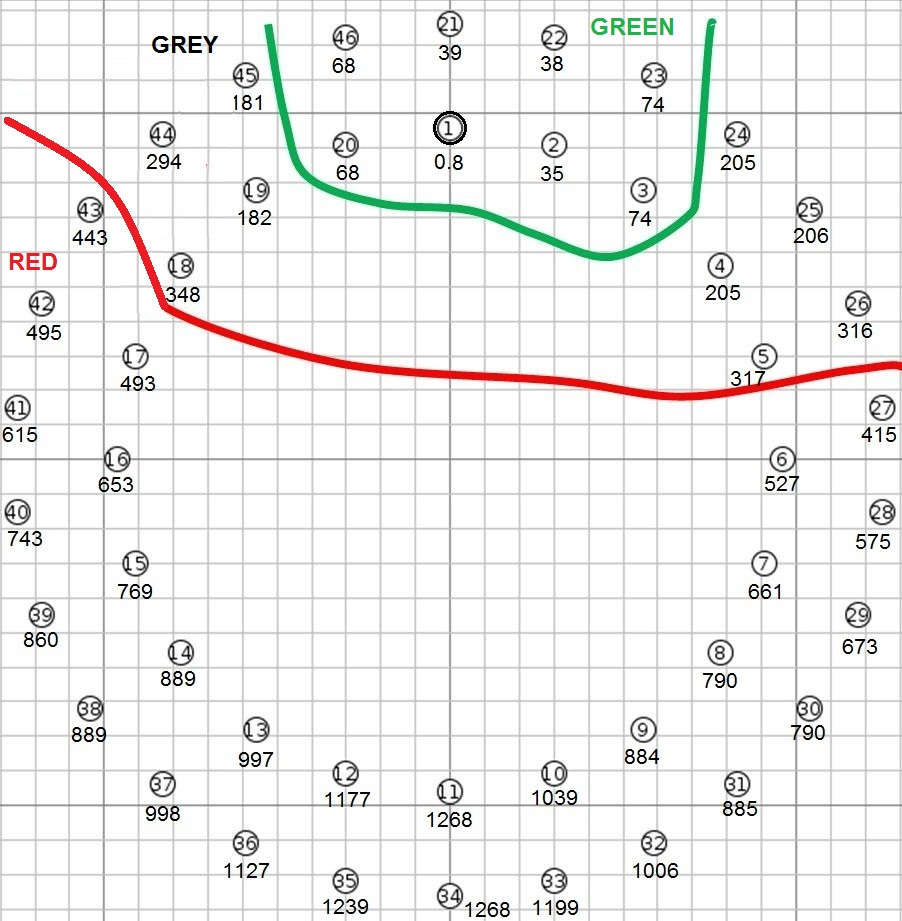
\includegraphics[width=.8\linewidth]{DoubleRingZ}
        \caption{IWS of intrusion initiated at each node and placement of nodes in Double Ring Topology}
% IWS measured under what circumstance? An update initiated from each node? There's no context as to what the data means.
% <Ash>  Correctly pointed out
        \label{fig:elliptopo} 
    \end{figure}

Figure~\ref{fig:elliptopo} shows the placement of the motes with mote ID written at the centre and IWS beneath the tiny circle.
The motes represented an intrusion point in the process of measuring IWS using Equation~\ref{eqn2}.
The IWS increases linearly with the increase in distance from the sink.
If the IWS in a network is organised in a specific order, e.g., chronologically  along some shape, 
% <dme> which specific order? Do you mean "sorted"? If so, say so: there are many potential specific orders...
% <Ash> chronologically
it would represent the original topology in some fashion.
For example, in the double ring topology, the circles are represented by the bimodal curve formed from the IWS represented by columns in Figure~\ref{fig:ellipgraph}.
\begin{figure}[t]
	\centering
        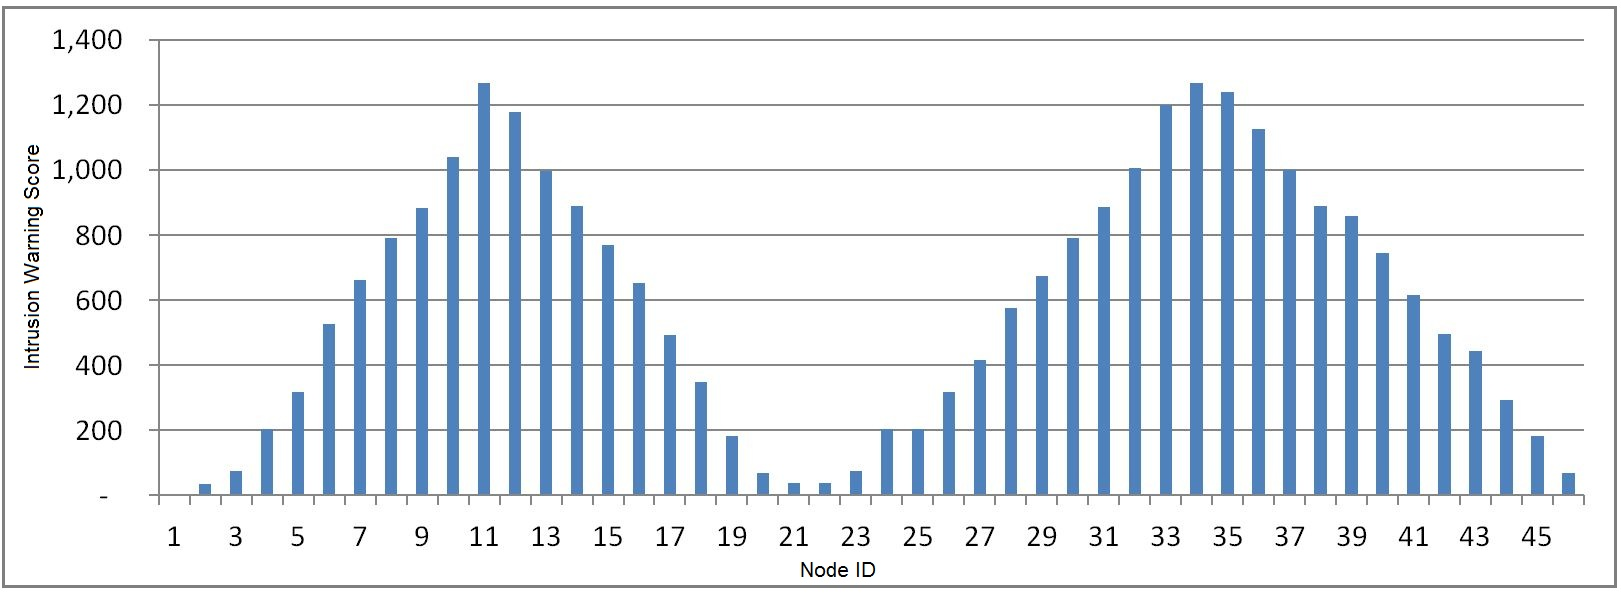
\includegraphics[width=\linewidth]{DR_Column}
        \caption{Comparison of IWS of intrusion initiated at different motes}
        \label{fig:ellipgraph}
\end{figure}

The main contribution of this research comes from the ability to report anomalies in terms of the quantitative IWS measure.
% <dme> I'm not sure that this is much of a contribution---the related work will have done this already, no? I've thought of IWS as being more of a statistical and simulator warm-up exercise before tackling decentralised detection, etc.
% <Ash> I do not knwo how to represent the IWS then. other may have similar contribution as well, doe it restrict me to suggest another option. Well, a comparison would be really good.
For example:  a regular legitimate update, initiated from node ID 1, resulted in a IWS of 0.8.
This result matches the theoretical expectation of very low IWS.
In addition to this, for intrusion scenario simulated from the nodes near the sink, the IWS was still fairly low (e.g.\ at mote ID 2, 3, 20--23, and 46). 
Because the IWS of the motes close to the sink is likely to be very low, it is quite difficult to conclude if such an IWS indicates an intrusion.
This area is marked as being within the GREEN zone, and needs to be adequately secured with additional physical security as intrusion in these motes is not easily detectable by the IDS.
For other motes, such as mote ID 4, 5, 24--26, 18, 19, 44 and 45, the IWS is neither too low, nor too high to be considered an intrusion. The area is marked as GREY to indicate the requirement of additional monitoring to reduce false positive cases.
However, for the distant motes--marked in the RED zone, the IWS is quite high and the IDS can conclude such cases are intrusions, such as the IWS of 1268 for mote ID 34, and 885 for mote ID 31. %,and likewise indicate intrusion.
Accordingly, Figure~\ref{fig:elliptopo} and~\ref{fig:ellipgraph} shows the region boundaries and thresholds of GREEN, GREY and RED zones.%

\begin{table*}[t]
\centering
\begin{tabular}{|l|*{17}{r|}r|}
\hline
\bd{Node ID}           & \bd{1} & \bd{4} & \bd{10} & \bd{12} & \bd{13} & \bd{15} & \bd{16} & \bd{18} & \bd{27} & \bd{31} & \bd{34} & \bd{36} & \bd{37} & \bd{38} & \bd{39} & \bd{40} & \bd{41} \\%& \bd{44}\\
%Mote ID           & 1 & 2 & 3 & 4 & 5  & 6 & 7 & 8 & 9 & 10 & 11 & 12 & 13 & 14 & 15  & 16 & 17 & 18 & 19 & 20 \\
\hline
\bd{Update Time}  &   404 	&  588 	& 170 	& 66 	& 16 &	 16 	& 65 &	 204 &	 526 & 329 &	 113 &	 66 &	 15 	& 16 	& 16 &	 65 &	125 \\%& 277 \\
\hline
\end{tabular}
\caption{Mote update time for intrusion at node 14 in Double Ring topology (partial data presented)}

\label{tab:dr_time_14}
\end{table*}

\begin{table*}[t!]
\centering
\begin{tabular}{|l|*{20}{r|}r|}
\hline
\bd{Node ID}           & \bd{1} & \bd{2} & \bd{3} & \bd{4} & \bd{5} & \bd{6} & \bd{7} & \bd{8} & \bd{9} & \bd{10} & \bd{11} &  \bd{33} & \bd{34} & \bd{35} & \bd{36} & \bd{37} & \bd{38} \\
%Mote ID           & 1 & 2 & 3 & 4 & 5  & 6 & 7 & 8 & 9 & 10 & 11 & ...& 31 & 32 & 33  & 34 & 35 & 36 & 37 & 38 \\
\hline	%	\hline

Power 100\%	   & 512 & 529 & 512 & 512 & 512  & 512 & 476 & 478 & 476 & 459 & 458 & 53  & 48 & 49 & 51 & 47 & 29 \\
%\hline

Power 50\%	  &31 & 59&254& 31& 31 &283& 32& 32& 254& 31 &253 &  31  & 30 & 31 & 31 & 30 & 0 \\
\hline
\end{tabular}
\caption{IWS from intrusion at motes in Owheo WSN (partial data presented). Further explained in Figure~\ref{subfig:owheo_full} and Figure~\ref{subfig:owheo_half}. }
\label{tab:owheo}
\end{table*}


The IDS can also detect the source of intrusion by analysing update time of all motes. %and its extent. 
For example, Table~\ref{tab:dr_time_14} shows the update time recorded at different motes when intrusion was initiated from note 14.
The timing data shows that lowest timing was recorded at node 13, 15, 37, 38, and 39 which was $\approx$16 seconds.
Node 14 did not report any time because of three reasons: 
\begin{inparaenum}
\item node 14 initiated the update, so it was updated at $0$ seconds;
\item it acted as a sink, the protocol did not require it to notify update time; and 
\item it is the compromised node whose protocol is expected to be altered.
\end{inparaenum}
From the timing data, the IDS can conclude that node 14 was the intrusion point.
The extent of intrusion, as specified earlier, is found out from reported version information.


%The idea of zoning associated with the IWS is very beneficial in securing a WSN.
The idea of zoning associated with the IWS is useful in designing secure WSN deployments. %, which is considered to be another major contribution of the work.
A network is more secure when it has a smaller GREEN and GREY zone, which implies that fewer resources will be needed to strengthen the security of these motes. %impenetrably secure less number of motes.
%Similarly, a smaller or non-existent GREY zone would require lesser monitoring measures.
%Such a secure WSN can be designed by varying the parameters like power level or even by physically relocating some motes.
Obtaining a real world scenario by varying different sets of design parameters such as power levels or position of nodes is an impossible task even for a small WSN.
% <dme> I have no idea what you're talking about in the previous sentence. <Ash> ki likhbo
The simulation environment used to design the IDS can be effectively utilised to obtain the expected IWS score range for different sets of parameters and then rank the sets based on how effectively they produce IWS values. 
However, any change in topology or design parameters, like power level, will require recalibrating the IDS. 
For example, we have simulated the set of IWS outcomes within the `Owheo Sensor Network' 
at two different power levels to investigate improving the security of our WSN using the IDS.

Table~\ref{tab:owheo} shows the IWS at different motes within the Owheo WSN as intrusion points at 100\% and 50\% power levels. 
%Here, mote ID 38 was marked as the sink.
At 100\% power level, %19 nodes were in GREEN zone, only one node in GREY zone and the rest 
only 16 nodes are in the RED zone.
When the same deployment is simulated at 50\% power level, %only seven nodes were in GREEN zone, two nodes were in GREY zone and rest 
27 motes are in the RED zone.
The deployment and the zoning boundaries at 100\% and  50\% power level have been shown in Figure~\ref{subfig:owheo_full} and~\ref{subfig:owheo_half} respectively.
Comparing the scenarios, it can clearly be established that deployment at 50\% power level is more secure than the other for two reasons:
\begin{inparaenum}
\item it has a GREEN and GREY zone of smaller size; and 
\item there are fewer nodes in these zones. 
\end{inparaenum}

\begin{figure}[t]
	\centering
        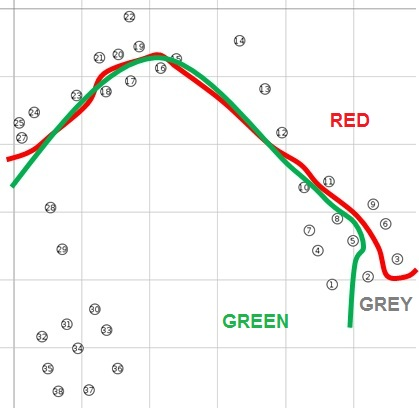
\includegraphics[width=.9\linewidth]{Owheo_full}
        \caption{Zone boundary at full power level}
        \label{subfig:owheo_full}
\end{figure}

\begin{figure}[t]
	\centering
        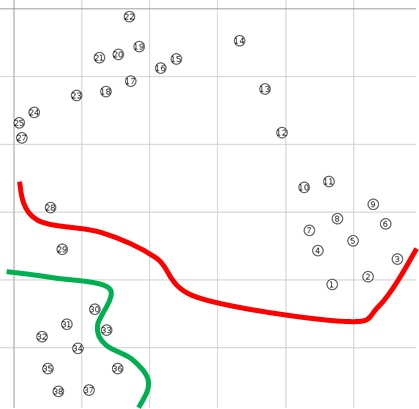
\includegraphics[width=.9\linewidth]{Owheo_half}
        \caption{Zone boundary at half power level}
% <dme> I fixed the odd capitalisation in both captions. I'm not sure why initial caps were used?
        \label{subfig:owheo_half}
\end{figure}



%\begin{figure*}[t!]
%    \centering
%    \begin{subfigure}[b]{0.5\textwidth}
%        \centering
%        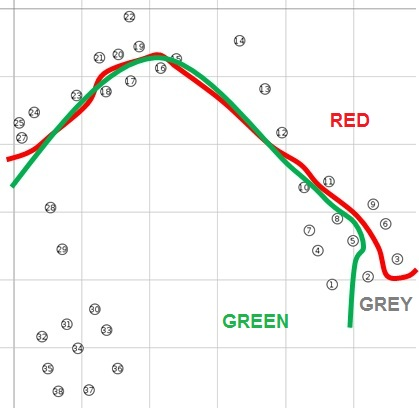
\includegraphics[height=2.5in]{Owheo_full}
%        \caption{Zone boundary at Full Power Level}
%        \label{subfig:owheo_full}
%    \end{subfigure}%
%    ~ 
%    \begin{subfigure}[b]{0.5\textwidth}
%        \centering
%        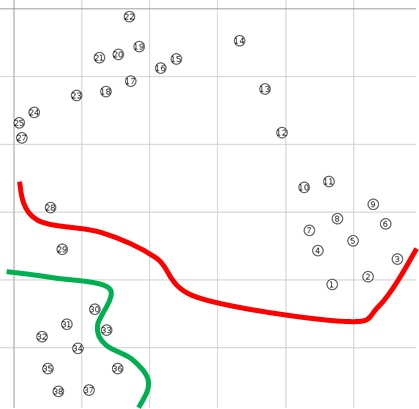
\includegraphics[height=2.5in]{Owheo_half}
%        \caption{Zone boundary at Half Power Level}
%        \label{subfig:owheo_half}
%    \end{subfigure}
%    \caption{Comparison of Zone boundary for power level variations in `Owheo Sensor Network'. IWS of the motes at the power levels are shown in Table~\ref{tab:owheo}}
%\label{fig:owheo}
%\end{figure*}


\section{Conclusion}
\label{sec:concl}

In this paper, we modelled an IDS solution to detect intrusions in WSNs during OTA software update.
We discussed the potential dangers associated with such updates.
The IDS is hosted on a server that remains physically connected to the  sink. 
% The sink has an ITC application which in coordination with the IDS performs the detection activity.
% <dme> ITC needs to be explained if included in the conclusion. Doesn't seem high value though. <Ash> okay
The system watches over the timing of software update patterns using a modified version of the Deluge protocol.
%Whenever a mote is updated, it sends an update related information to designated sink using a datagram.  
%Related information from the datagram is filtered by the ITC for further processing at IDS.

The first contribution of the research is in quantifying intrusion through an IWS that indicates the location and extent of intrusions.
%The IWS is a quantitative indicator of possible intrusion.
%The utility function that computes IWS is designed to neutralise the undesired %/unexpected
%changes in mean and standard deviation which are expected to contribute to a near zero IWS.
The other important contribution is related to designing secure WSNs using the IWZ metric as a guide.
%classifying expected IWS into zones.
%The concept of zoning using the IDS is a very useful tool in designing secure WSN deployment.
%The IDS can be used to simulate all possible combinations of parameters and  to rank the sets based on intrusion vulnerability.
%For example, a WSN with known small insecure zone is much easier to protect than a larger zone.
%The ranking mechanism is useful in such scenario.
The IDS also can indicate some other kinds of anomalies such as node relocation, node repudiation or node compromise.

The proposed technique has several limitations. 
It assumes some special situations, such as a static WSN with a single sink.
It also assumes that network-wide information will not be forged. %to have network wide transparent knowledge.
These assumptions may not hold in a real WSN and can be addressed in a more realistic way using a decentralised technique, which we plan to experiment in future.
% <dme> OK, so what are you planning to do in future to address this? Readers will want to know. <Ash> decentralised approach
In addition to this, assumptions about the attacker are: the attacker can employ enough resources to break into the cryptographic protections within the sensors; however, he is not able to modify the protocols in an uncompromised sensor.
The IDS has an obvious functional limitation.
It cannot identify an intrusion in certain scenarios such as 
%For example, when an intrusion takes place 
in the close vicinity of the sink.%, this IWS may not always be sufficiently large to be identified as an intrusion.
The other limitation stems from the fact that the results are based on simulated data and need support from real world implementation.
In future,  the IDS can be implemented to examine real world performance including cases of multiple sinks with mobile sensors.


% \section{References}
% References should be in the standard author-date format, examples of which are shown below (shown is a conference paper, a thesis, a book, a book section and a journal paper in that order).  The required formats can be obtained by including the {\it natbib} package and using style {\it agsm}.  The files {\tt natbib.sty} and {\tt agsm.bst} are available at the CRPIT website.  The  {\it harvard} package, which is also available, can also be used as an alternative to natbib.

\bibliographystyle{agsm}    % or some other suitable package.
\bibliography{auspdc}


\end{document}


%  LocalWords:  Ashraful Alam aalam dme uncompromised Cooja Contiki
